\documentclass[11pt,english,a4paper]{article}
\usepackage{natbib, amsmath, amsfonts, units, graphicx, hyperref, txfonts, fleqn, geometry, pifont, setspace}
% \usepackage{lmodern}
\usepackage{fancyhdr}

\providecommand{\keywords}[1]{\textbf{\textit{Keywords ---}} #1}
\renewcommand*{\bibfont}{\small}
\setlength{\bibsep}{0.0pt}

\pagestyle{fancy}
\fancyhf{}
\lhead{Smith LS and Liang Q (2013)}
\rhead{}
\cfoot{\thepage}

\title{Towards a generalised GPU/CPU shallow-flow modelling tool}
\author{Luke S. Smith,\\
	Civil Engineering and Geosciences,\\
	Newcastle University,\\
	Newcastle upon Tyne,\\
	NE1 7RU UK\\
	\texttt{l.s.smith@ncl.ac.uk}
	\thanks{Telephone: +44 (0) 191 208 8599}
\and
	Qiuhua Liang,\\
	Civil Engineering and Geosciences,\\
	Newcastle University,\\
	Newcastle upon Tyne,\\
	NE1 7RU UK\\
	\texttt{qiuhua.liang@ncl.ac.uk}
}
\date{\vspace*{12.0pt}Accepted \textbf{17 September 2013} \\ Published \textbf{15 December 2013}}

\begin{document}
\maketitle


\begin{abstract}
This paper presents new software that takes advantage of modern graphics processing units (GPUs) to significantly expedite two-dimensional shallow-flow simulations when compared to a traditional central processing unit (CPU) approach. A second-order accurate Godunov-type MUSCL-Hancock scheme is used with an HLLC Riemann solver to create a robust framework suitable for different types of flood simulation. A real-world dam collapse event is simulated using a 1.8 million cell domain with CPU and GPU hardware available from three mainstream vendors. The results are shown to exhibit good agreement with a post-event survey. Different configurations are evaluated for the program structure and data caching, with results demonstrating the new software's suitability for use with different types of modern processing device. Performance scaling is similar to differences in quoted peak performance figures supplied by the vendors. We also compare results obtained with 32-bit and 64-bit floating-point computation, and find there are significant localised errors introduced by 32-bit precision.
\end{abstract}
\keywords{shallow water equations, graphics processing units, Godunov-type scheme, flood modeling, high-performance computing}

\vfill
\noindent\fbox{
\begin{minipage}{\dimexpr\textwidth-2\fboxsep-2\fboxrule}
\small
This is the authors' version of a work that was accepted for publication in Computers \& Fluids. A definitive version was subsequently published in Computers \& Fluids, 88:334-343. doi:\url{http://dx.doi.org/10.1016/j.compfluid.2013.09.018}
\end{minipage}
}

\section{Introduction}

Free-surface shallow-flow models can be applied across a wide range of scenarios to simulate flood events, tsunami, and the consequences of dam collapse. Amongst the most advanced models are Godunov-type schemes, allowing accurate simulation even where complex flow dynamics exist (e.g. hydraulic jumps), and utilising high-resolution datasets available at low expense with LiDAR data. Auspicious engineering design and risk analysis increasingly demands these high levels of detail and accuracy \cite{French_03,Haile_05,Marks_00}. To capture highly transient complex hydrodynamic processes, e.g. those induced by dam breaks, a Godunov-type scheme is normally developed using an explicit scheme in time integration, which imposes a strict constraint on the timestep. However, these explicit time-marching schemes are computationally expensive, thus high-resolution simulations across large catchment or city scales are often unfeasible in practice without super-computers, despite recent substantial developments in CPU power. This deficiency is especially pertinent for natural flood management techniques, whereby small runoff storage and attenuation features are distributed throughout a catchment, as shown to be effective in pilot projects in small catchments such as Belford, Northumberland \cite{EnvironmentAgency_12,Wilkinson_10}. Computational models do not yet exist with sufficient physical basis to scientifically elucidate the practice and establish how to upscale the approach to much larger catchments. New approaches are required which can expedite simulations without compromising the numerical representation of the underlying physical processes, if we are to provide the necessary scientific basis, understanding, and guidance for applying this cost-effective approach elsewhere. 

To overcome computational constraints, numerous types of acceleration have been explored previously. Simplification of the numerical representation often provides inaccurate velocities, therefore compromising the temporal accuracy of the solution \cite{Pender_10,Singh_96,Neelz_09}, and may neglect important phenomena such as backwater effects; dynamic grid adaptation delivers limited benefits (2-3x faster) for complex flow characteristics and introduces challenges for managing mass and momentum conservation during refinement \cite{Liang_04}; many high-performance computing (HPC) techniques such as distributed computing (e.g. Condor) are constrained by communication because of the interdependency of the solution between cells and their neighbours, making scalable implementations difficult to accomplish \cite{Pau_06,Delis_09}. 

A more promising technique involves graphics processing units (GPUs), which are commonplace for gaming systems but were only recently exposed for exploitation in scientific computing \cite{Owens_07,Nickolls_10}. Compared to central processing units (CPUs), there are typically many more processing elements (i.e. cores, compute units) in GPUs. They are ideal for repetitive calculations across large datasets, but there are numerous additional constraints to consider if high performance levels are to be achieved. Successful GPU-computed models have already been applied in computational fluid dynamics (CFD) for astrophysics, magneto-hydrodynamics, haemodynamics and gas dynamics (e.g. \cite{Bisson_12}). A GPU designed for scientific use can be expected to boost performance by approximately 6.7 times compared to the typical quad-core CPU device used herein with 64-bit floating-point computation, and assuming architecture-efficient implementations \cite{Intel_12,NVIDIA_11}. Importantly however, performance benefits can scale with multiple devices \cite{Kuo_11,Saetra_12}. Advantages are evident across a wide range of different approaches, numerical schemes and spatial discretisations (e.g. \cite{Kuo_11,Horvath_10,Wang_10,Rossinelli_11,Schive_11,Crespo_11}). Suitability and successful application for the shallow-water equations is evidenced with both a Kurganov-Petrova scheme and split HLL method \cite{Brodtkorb_10,Brodtkorb_10a,Brodtkorb_11,Saetra_12,Kuo_11}, however current literature focusses on Riemann solver-free schemes, 32-bit floating-point, and vendor-specific implementations (primarily CUDA). Computationally intensive schemes of higher orders in time using more generalised Riemann solvers which consider contact and shear waves, are worthy of further research. 

GPUs provide an excellent ratio of computing power to cost, making them a potential future tool for engineering consultancies, but commercially viable software must be resilient to hardware differences in capacities and architectures. An appropriate scheme for application across a wide range of scenarios must also be able to preserve depth positivity, capture shocks (flow discontinuities), appropriately manage wet-dry interfaces, and handle complex domain topography or exhibit the so-called well-balanced property \cite{Xing_10,Murillo_10}. 

Few generalised modelling tools with all these qualities currently exist. Herein we develop software that does boast all of the aforementioned qualities to provide a next-generation shallow-flow modelling tool that can readily be applied for different purposes (i.e. different flood simulations and catchment modelling) and can easily be optimised for a wide range of different GPUs and CPUs without compromising on accuracy, functionality or the robustness of the solution. Through application to a real-world dam-break event, one of the most difficult types of flood scenario to accurately simulate, we demonstrate that high levels of performance are achievable even with a complex Godunov-type scheme and an HLLC Riemann solver. 

\section{Review of a finite-volume Godunov-type scheme}

The conservative form of the shallow water equations (SWEs) can be obtained by depth-integration of the Reynolds-averaged Navier-Stokes equation, to give a hyperbolic conservation law defined as
\begin{equation}
	\label{SWE}
	\frac{\partial\textbf{U}}{\partial t} +
	\frac{\partial\textbf{F}}{\partial x} +
	\frac{\partial\textbf{G}}{\partial y} =
	\textbf{S} ,
\end{equation}
where \(\textbf{U}\) is a vector of conserved variables, \(\textbf{F}\) and \(\textbf{G}\) are vectors of fluxes in \(x\)- and \(y\)-directions, and \(\textbf{S}\) is a vector of source terms. The values of \(t\), \(x\), and \(y\) represent time and the two Cartesian coordinates respectively. Herein we neglect the viscous fluxes, surface stresses and Coriolis effects to give vectors
\renewcommand{\arraystretch}{1.5}
\begin{equation}
	\label{SWETerms}
	\begin{alignedat}{4}
		&\textbf U && = \left[ \begin{array}{c}
			\eta \\
			uh \\
			vh
		\end{array} \right] , ~ &&
		\textbf F &&  = \left[ \begin{array}{c}
			hu \\
			hu^2 + \frac{1}{2}(g\eta^2 - 2\eta z_b) \\
			huv
		\end{array} \right] ,\\
		&\textbf G && = \left[ \begin{array}{c}
			hv \\
			hvu \\
			hv^2 + \frac{1}{2}(g\eta^2 - 2\eta z_b) \\
		\end{array} \right] , ~ &&
		\textbf S && = \left[ \begin{array}{c}
			0 \\
			-\frac{\tau_bx}{\rho} - g\eta \frac{\partial z_b}{\partial x} \\
			-\frac{\tau_by}{\rho} - g\eta \frac{\partial z_b}{\partial y} \\
		\end{array} \right] .
	\end{alignedat}
\end{equation}
Here, \(\eta\) is the free-surface level above datum; \(u\) and \(v\) are depth-averaged velocities in the \(x\)- and \(y\)-directions respectively; \(h\) is the water depth; \(uh (=q_x)\) and \(vh (=q_y)\) are unit-width discharges; \(g\) is the acceleration due to gravity; \(\rho\) is the water density; \(\tau_{bx}\) and \(\tau_{by}\) are bed stresses in the two directions; and \(z_b\) is the bed elevation above datum. The deviatory vector forms displayed here ensure the equations exhibit the well-balanced property and thereby provide the correct behaviour for a lake-at-rest case with uneven bed topography \cite{Liang_09}.

\subsection{Finite-volume Godunov-type scheme}

A Godunov-type scheme \cite{Godunov_59} is used to solve \eqref{SWE} by computing fluxes through local Riemann solutions at each cell interface. Flux differences along each axis are then used to update flow variables in each cell with the time-marching formula, 
\begin{equation}
	\label{GodunovUpdate}
	\begin{alignedat}{2}
	\textbf{U}^{t+\Delta t} = \textbf{U}^t & - \frac{\Delta t}{\Delta x}(\textbf{F}^+ - \textbf{F}^-) 
					     &  - \frac{\Delta t}{\Delta y}(\textbf{G}^+ - \textbf{G}^-) + \Delta t \textbf{S} , 
	\end{alignedat}
\end{equation}
where \(\textbf{F}^-\), \(\textbf{F}^+\), \(\textbf{G}^-\), \(\textbf{G}^+\)  are fluxes through a cell's western, eastern, southern and northern interfaces respectively; and \(\Delta x\) and \(\Delta y\) are cell dimensions in each respective direction. The HLLC (i.e. Harten, Lax, van Leer, contact-restoration) solver \cite{Toro_94} is used for approximate Riemann solutions, with less computational burden than an exact solution but an appropriate degree of accuracy for most shallow flow simulations \cite{Erduran_02,Zoppou_03}.

A MUSCL-Hancock approach \cite{vanLeer_84} is adopted to achieve second-order accuracy in both space and time. Specifically, cell face-extrapolated values are obtained using a MUSCL linear reconstruction method implemented with a MINMOD slope limiter \cite{Roe_86} for flow variables \(\begin{matrix}[\eta & uh & vh]\end{matrix}^T\) to prevent spurious oscillations that might otherwise be introduced \cite{Toro_01}. The MINMOD limiter is selected herein because its properties provide better numerical stability for a wide range of conditions \cite{Suresh_00,Yee_06}.

\subsection{Depth positivity preservation}

Non-negative reconstruction is required before computing Riemann solutions to ensure depth positivity is preserved. The approach adopted herein is appropriate for flood modelling \cite{Liang_10}. In the context of a finite-volume Godunov-type scheme, after linear reconstruction of flow variables and the bed elevation for the cell interface under consideration, an intermediary bed elevation is obtained, where \(\tilde{ }\) denotes a variable before non-negative reconstruction and subscript \(L\) or \(R\) denote sides of the interface,
\begin{equation}
	\label{NonNegRec1}
	\hat{z}_b = max(\tilde{z}_{b,L}, \tilde{z}_{b,R}) ,
\end{equation}
from which the final reconstructed variables can be computed at both sides of the interface. Velocities are unchanged and used to compute new unit-width discharge with the reconstructed depth and free-surface level,
\begin{equation}
	\label{NonNegRec2}
	\begin{alignedat}{2}
		&h && = max(0, \tilde{\eta} - \hat{z}_b) ,\\
		&\hat{\eta} && = h + \hat{z}_b .
	\end{alignedat}
\end{equation}
Finally, a local bed modification is applied to datum-dependent variables to ensure the free-surface level is not below the bed elevation \cite{Liang_10},
\begin{equation}
	\label{NonNegRec3}
	\begin{alignedat}{2}
		&\Delta z && = max(0, \hat{z}_b - \tilde{\eta}_L) ,\\
		&z_b      && = \hat{z}_b - \Delta z               ,\\
		&\eta     && = \hat{\eta} - \Delta z              .
	\end{alignedat}
\end{equation}
The reconstructed flow variables resulting from \eqref{NonNegRec2} and \eqref{NonNegRec3} together with the unit-width discharges become the states defining the local Riemann problem across the cell interface, which is subsequently solved using an HLLC approximate Riemann solver to give the interface fluxes for updating the flow variables to a new time step using \eqref{GodunovUpdate}.

\subsection{Stability criterion}

The maximum permissible timestep for stability in the scheme is governed by the work of Courant-Friedrichs-Lewy \cite{Courant_67} and given by lowest instance from all cells of
\begin{equation}
	\label{CFL}
	\Delta t = C \cdot min \left[\frac{\Delta x}{\lvert u + \sqrt{gh} \rvert} , \frac{\Delta y}{\lvert v + \sqrt{gh} \rvert}\right] ,
\end{equation}
where \(C\) is the Courant number, with constraint \(0 < C \le 1\). The Courant number is set to 0.5 for simulations herein. 

\subsection{Implicit friction solution}

A point-implicit scheme is given through Taylor expansion of an ordinary differential equation accounting for friction effects \cite{Liang_10}. This approach allows for a solution which is independent of the Godunov-type scheme. Neglecting higher-order terms in the expansion, unit-width discharges after accounting for friction become
\begin{equation}
	\label{Friction}
	\begin{alignedat}{3}
		&q_{x}^{t+\Delta t} && = q_{x}^{t} + \Delta tF_x && ,\\
		&q_{y}^{t+\Delta t} && = q_{y}^{t} + \Delta tF_y && ,\\
	\end{alignedat}
\end{equation}
where for axis \(a\) and perpendicular axis \(b\),
\begin{equation}
	\label{FrictionPrereq}
	\begin{alignedat}{2}
		&F_a      && = \frac{S_{fa}}{D_{da}} ,\\
		&S_{fa}   && = -q_a\frac{C_f}{h^2}\sqrt{q_{x}^{2} + q_{y}^{2}} ,\\
		&D_{da}   && = 1 + \Delta t \times \frac{C_f}{h^2} \times \frac{2q_a + q_b}{\sqrt{q_{x}^{2} + q_{y}^{2}}} ,\\
		&C_f      && = \frac{gn^2}{h^{\frac{1}{3}}} .
	\end{alignedat}
\end{equation}

\section{GPU-based implementation}

\begin{figure*}[tb]
\centering
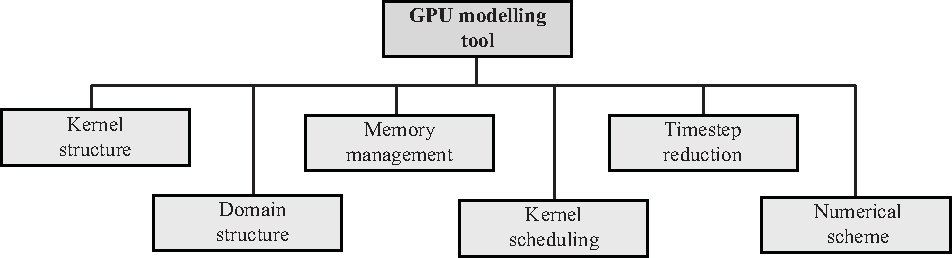
\includegraphics[width=0.85\textwidth]{Figure_1_Greyscale.pdf}
\caption{Main considerations for designing the shallow-flow modelling tool.}
\label{ModelComponents}
\end{figure*}

Godunov-type schemes have successfully been applied in a wide range of literature, but computational power has limited applications for extremely large domains with high-resolution representation. GPU computing offers a new and revolutionary means to achieve this, further advancing shallow-flow modelling practice. The Open Computing Language (OpenCL) is a consortium-led project involving multiple hardware vendors that allows developers to produce low-level code compatible with a variety of modern CPUs, GPUs and APUs available from NVIDIA, AMD and Intel \cite{KhronosOpenCL_12,NVIDIA_10,AMD_11}. The software developed herein uses OpenCL to provide the greatest compatibility between different device and hardware configurations, whilst the performance levels achievable are comparable to popular alternatives such as CUDA \cite{Fang_11}. Non-parallelised parts of the software were developed in C++. Differences in architecture, quantity of, and structure of compute units, and memories available thereon make it difficult to design code which can be considered optimised across a large number of devices. A new model structure is presented in this work to cope with these difficulties, and variations in memory management are assessed to determine their effect.

Successful and efficient implementation for GPUs requires careful consideration of the six elements shown in Fig. \ref{ModelComponents}, where a kernel refers to a discrete function within the program that can be executed in parallel across a range of data, and a reduction entails identifying a single value (e.g. minimum, maximum, or sum) from a large number of elements. To address hardware differences properly, the software developed allows end-user configuration of floating-point precision, workload balance in data reductions, and caching from global to local memory where applicable. Unlike existing software, a suitable and optimised configuration should therefore be achievable for any device conformant to the OpenCL specification.

\subsection{Domain structure}

A regular Cartesian grid of \(M \times N\) cells is used. This reduces the total data requirement and computational burden as no structure is necessary relating cells, and trigonometric functions are not required to update cells. Static cell data and initial conditions for transient variables are read from raster files using the Geospatial Data Abstraction Library (GDAL), thereby providing support for most common GIS file formats. Device-specific binaries are compiled before each simulation with the system's OpenCL drivers, allowing pre-processor macros to define many constants including the domain dimensions. 

\subsection{Memory management}

\begin{figure*}[tb]
\centering
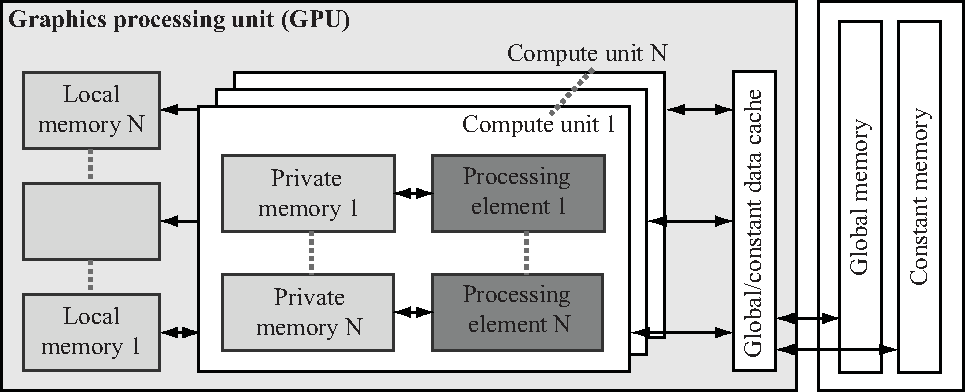
\includegraphics[width=0.7\textwidth]{Figure_2_Greyscale.pdf}
\caption{Memory model adopted in OpenCL, representing the structure of a GPU device and its global, local, private, and constant memory.}
\label{OpenCLStructure}
\end{figure*}
\begin{figure*}[tbh]
\centering
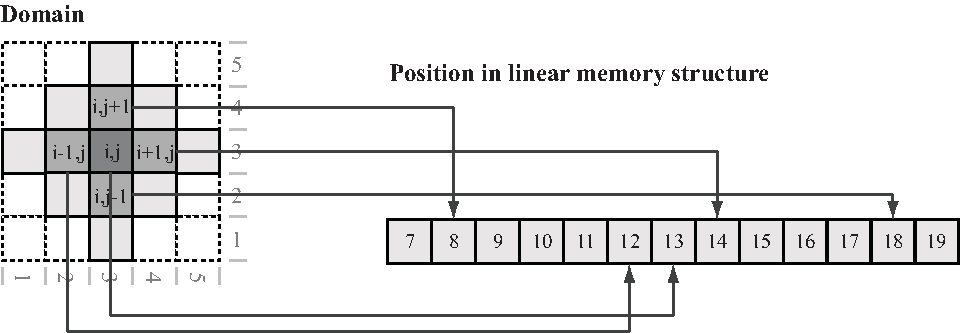
\includegraphics[width=0.8\textwidth]{Figure_3_Greyscale.pdf}
\caption{Requisite neighbour cell data to advance cell \(i,j\) demonstrating irregular strides when accessing global arrays.}
\label{RequisiteCellData}
\end{figure*}
\begin{figure*}[tbh]
\centering
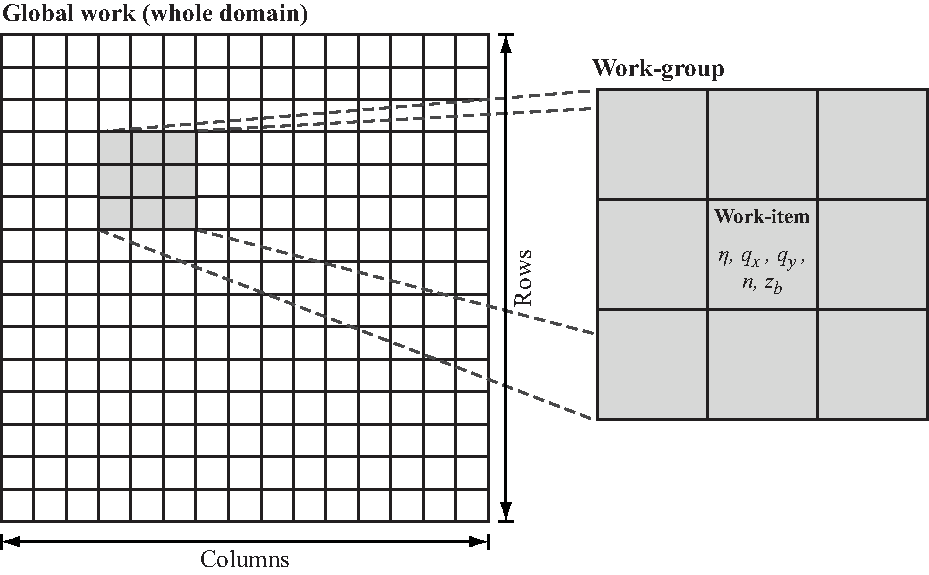
\includegraphics[width=0.7\textwidth]{Figure_4_Greyscale.pdf}
\caption{Structure of the OpenCL execution model as applied to the numerical scheme and domain structure herein.}
\label{OpenCLExecStructure}
\end{figure*}
\begin{figure*}[tbh]
\centering
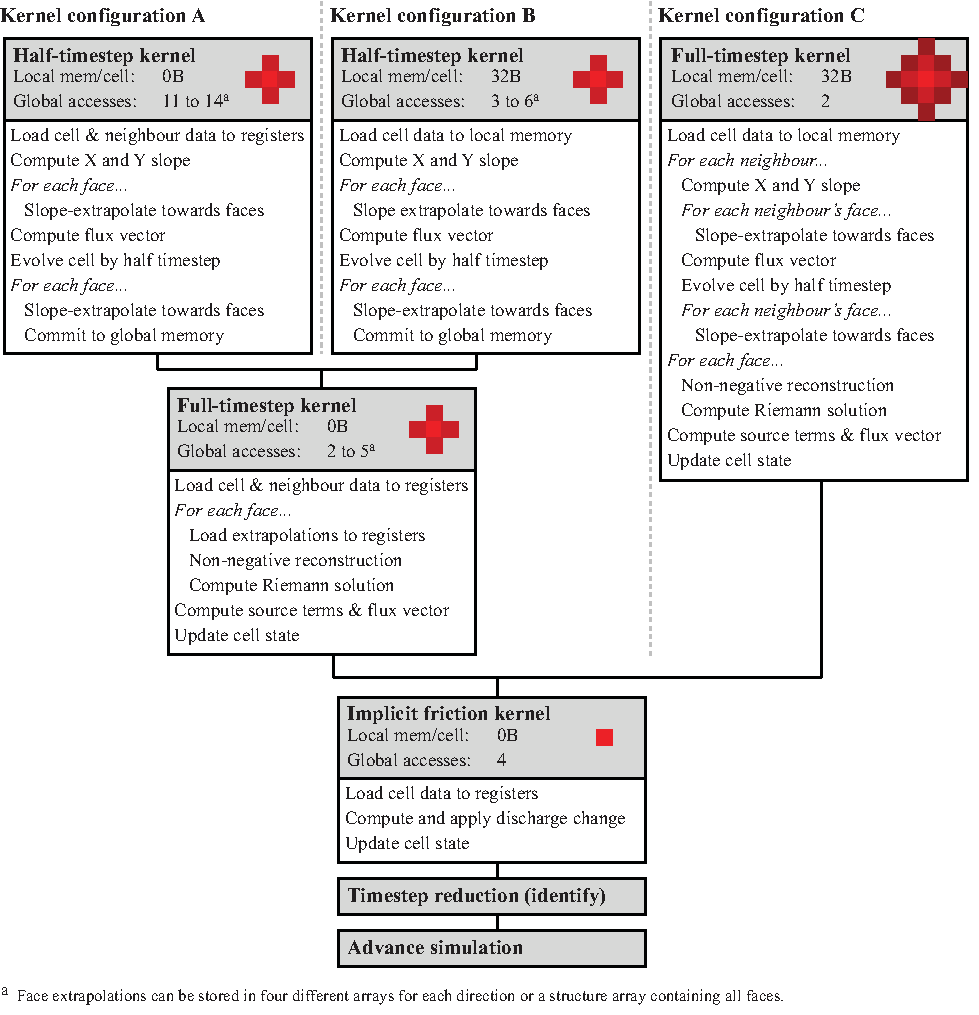
\includegraphics[width=0.8\textwidth]{Figure_5_Colour.pdf}
\caption{Implementation of the numerical scheme with three different kernel configurations intended to suit a majority of modern processing devices, and the data stencils for cell data required by each.}
\label{Kernels}
\end{figure*}
\begin{figure*}[tbh]
\centering
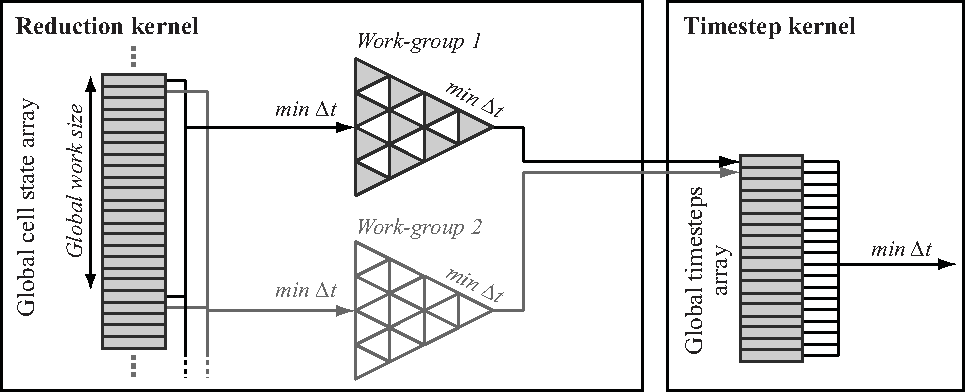
\includegraphics[width=0.75\textwidth]{Figure_6_Greyscale.pdf}
\caption{Simplified representation of the two-stage timestep reduction process, with only the first two work-groups indicated.}
\label{ReductionProcess}
\end{figure*}
\begin{figure*}[tbh]
\centering
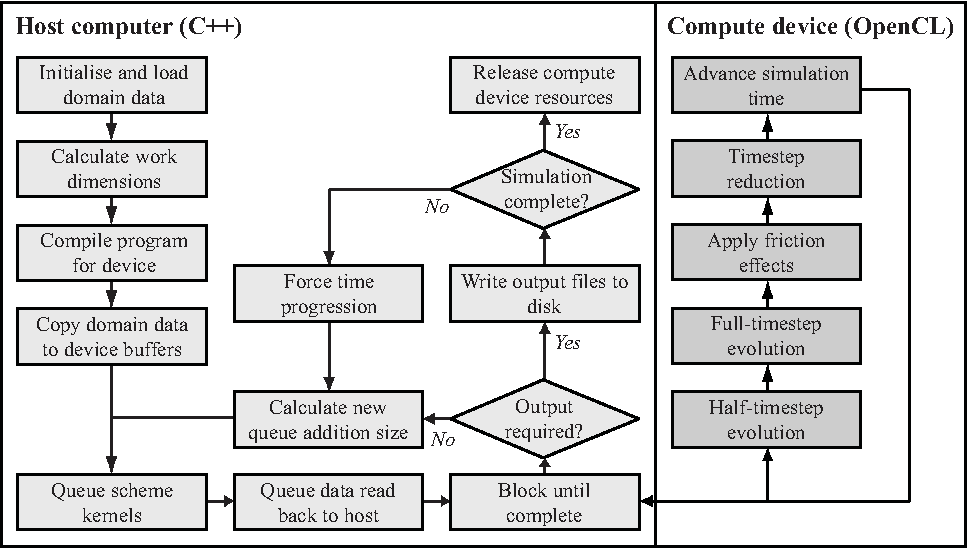
\includegraphics[width=0.7\textwidth]{Figure_7_Greyscale.pdf}
\caption{Flowchart of main operations on the host computer and compute device.}
\label{ComputerDeviceInteraction}
\end{figure*}
\begin{figure*}[tbh]
\centering
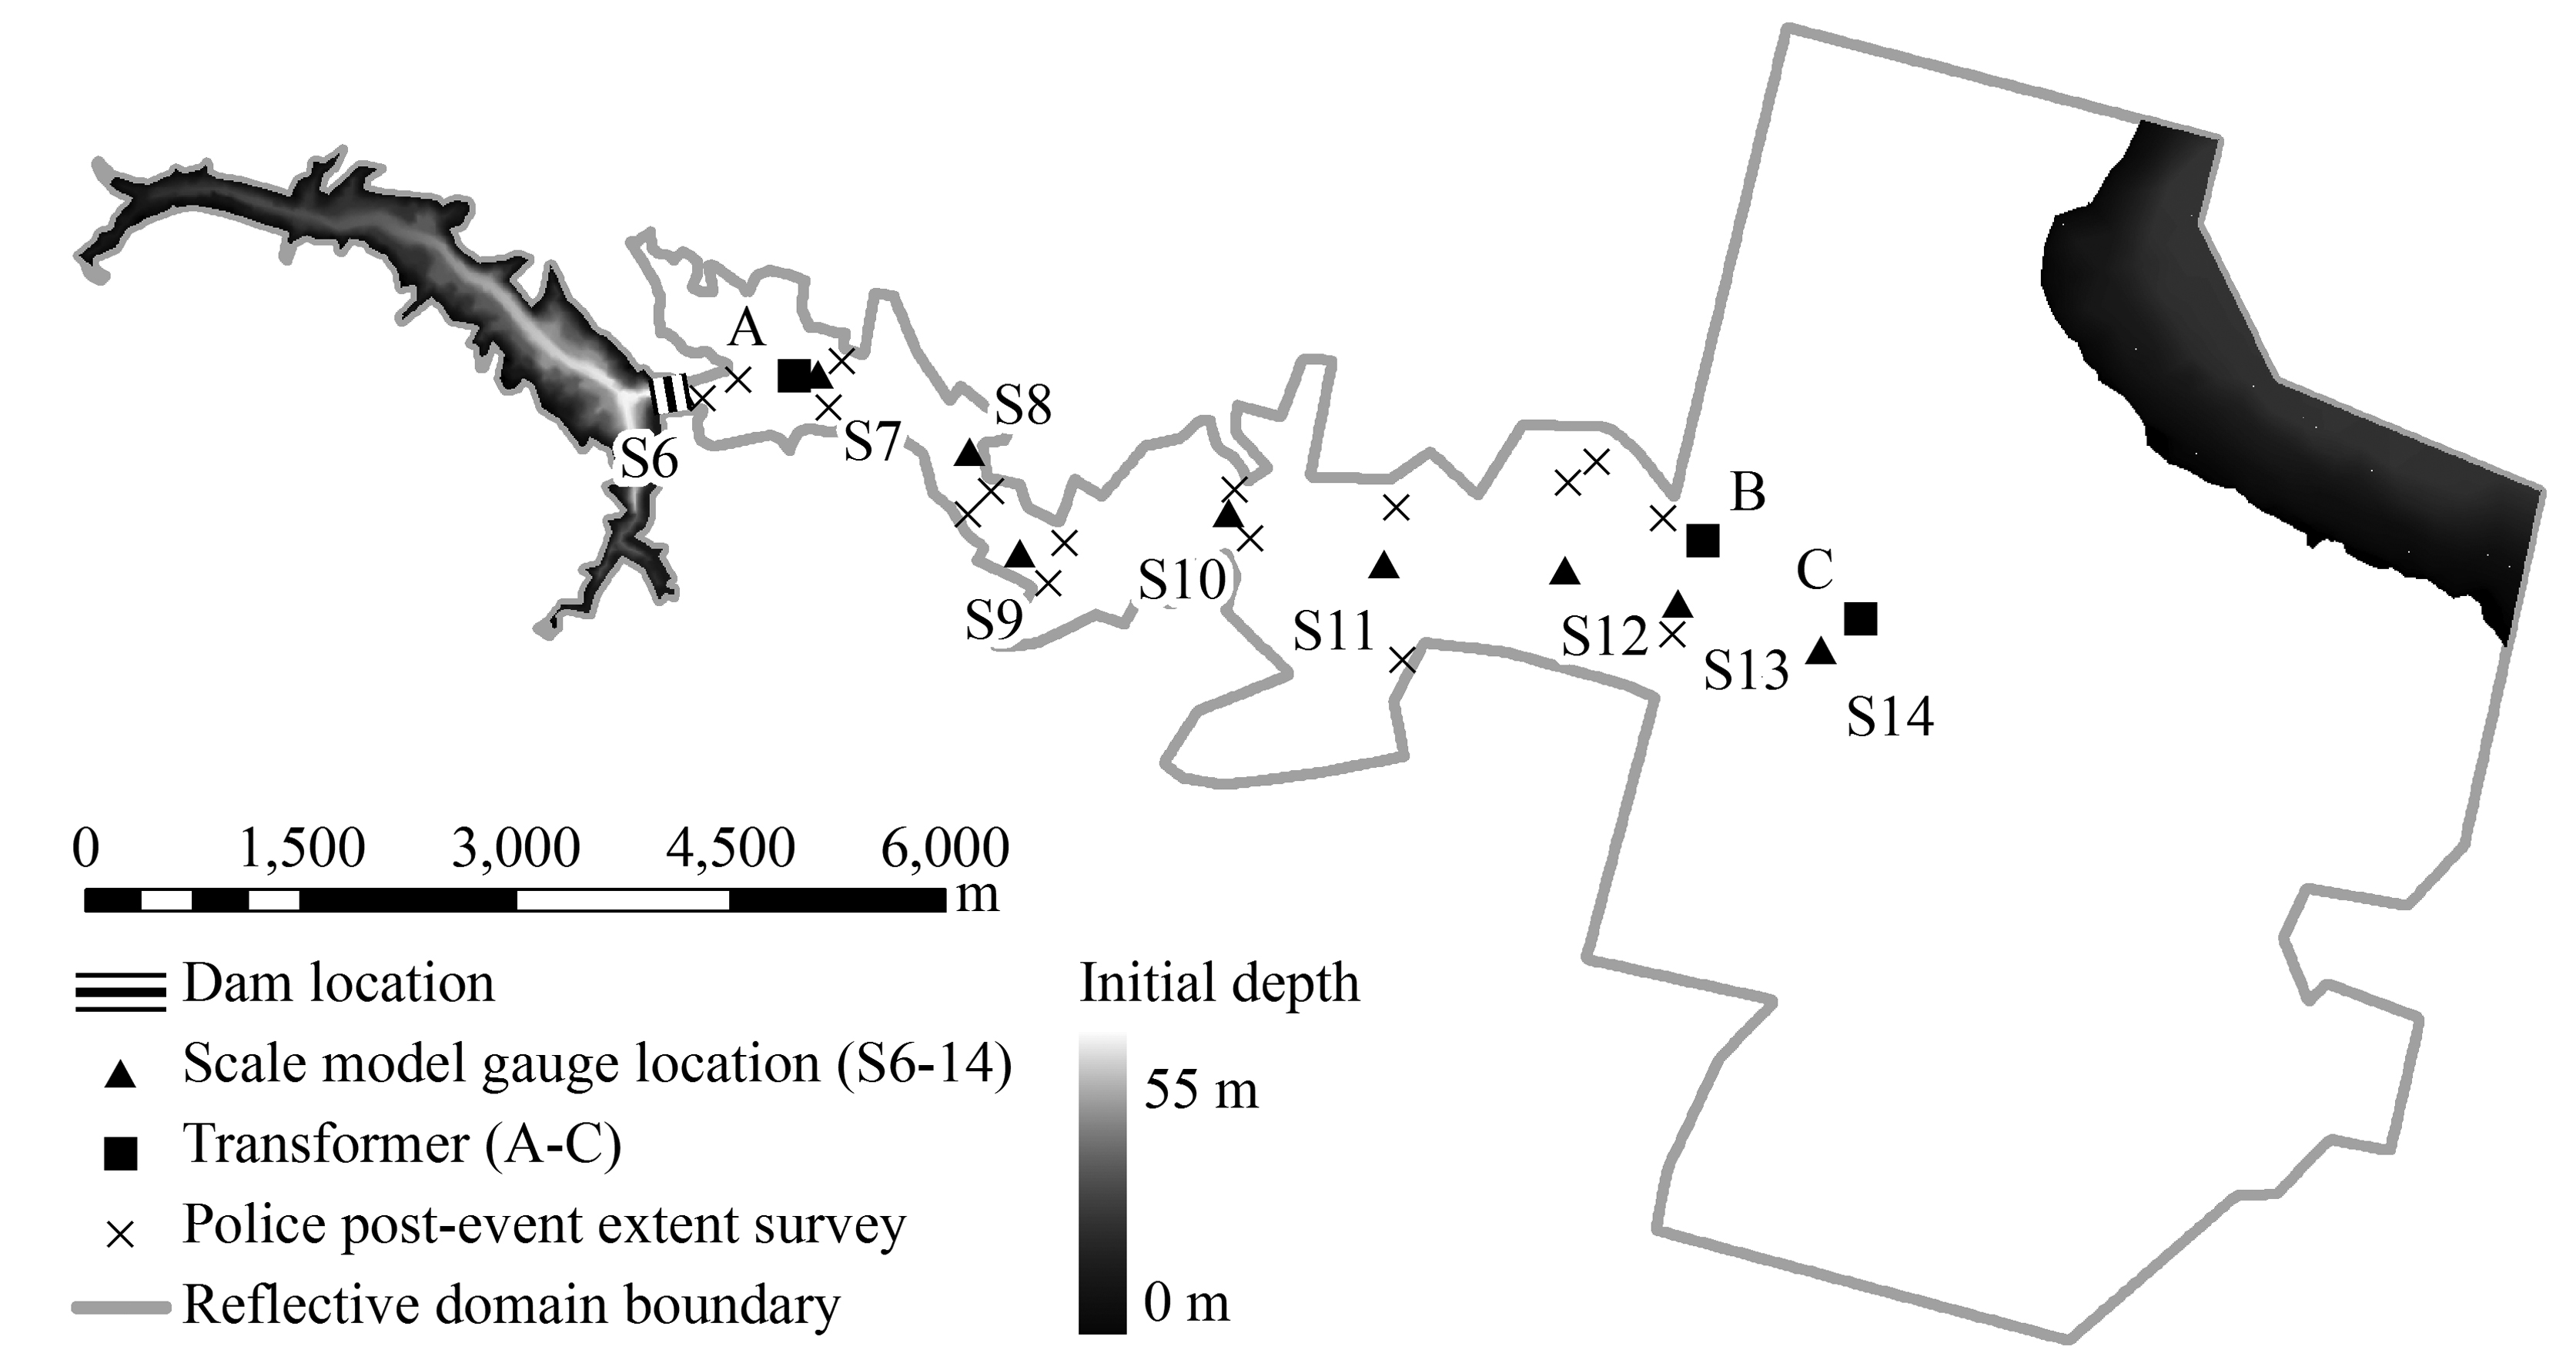
\includegraphics[width=0.75\textwidth]{Figure_8_Greyscale.jpg}
\caption{Malpasset dam-break domain, initial conditions and locations of validation points.}
\label{MalpassetIntro}
\end{figure*}
\begin{table*}[tbh]
\small
\centering
\caption{Total simulation time and cell calculation rate using three different devices, cache configurations and floating-point precisions.}
\label{PerformanceResults}
\makebox[\linewidth]{
\begin{tabular}{llrrrrrr}
\hline
			 		& 			& \multicolumn{2}{c}{AMD FirePro V7800}			& \multicolumn{2}{c}{NVIDIA Tesla M2075}			& \multicolumn{2}{c}{Intel Xeon E5-2609} 	\\
Kernel/cache	 		& Precision 	& Time (s) 	& Rate (x10\textsuperscript{6}/s) 	& Time (s) 	& Rate (x10\textsuperscript{6}/s)	& Time (s) 	& Rate (x10\textsuperscript{6}/s) 	\\
\hline
A: None 				& 32-bit 		& 84 			& 435	 		& 66 			& 556	 		& 821 		& 45	 \\
  					& 64-bit 		& 363 		& 106	 		& 243 		& 159	 		& 1534 		& 25	 \\
B: Normal				& 32-bit 		& 142 		& 258	 		& 125 		& 294	 		& 956 		& 38	 \\
					& 64-bit 		& 446 		& 86		 		& 381 		& 101	 		& 1730 		& 22	 \\
B: Oversized			& 32-bit 		& 122 		& 300	 		& 88 			& 417	 		& 951 		& 39	 \\
					& 64-bit 		& 442 		& 87		 		& 366 		& 105	 		& 1739 		& 22	 \\
C: Normal				& 32-bit 		& 122 		& 298	 		& 117 		& 314	 		& 1136 		& 32	 \\
					& 64-bit 		& 844 		& 45		 		& 576 		& 67		 		& 2818 		& 14	 \\
C: Oversized			& 32-bit 		& 110 		& 335	 		& 88 			& 417	 		& 1144 		& 32	 \\
					& 64-bit 		& 820 		& 47		 		& 554 		& 69		 		& 2881 		& 13	 \\
\hline
\end{tabular}
}
\end{table*}
\begin{figure*}[tbh]
\centering
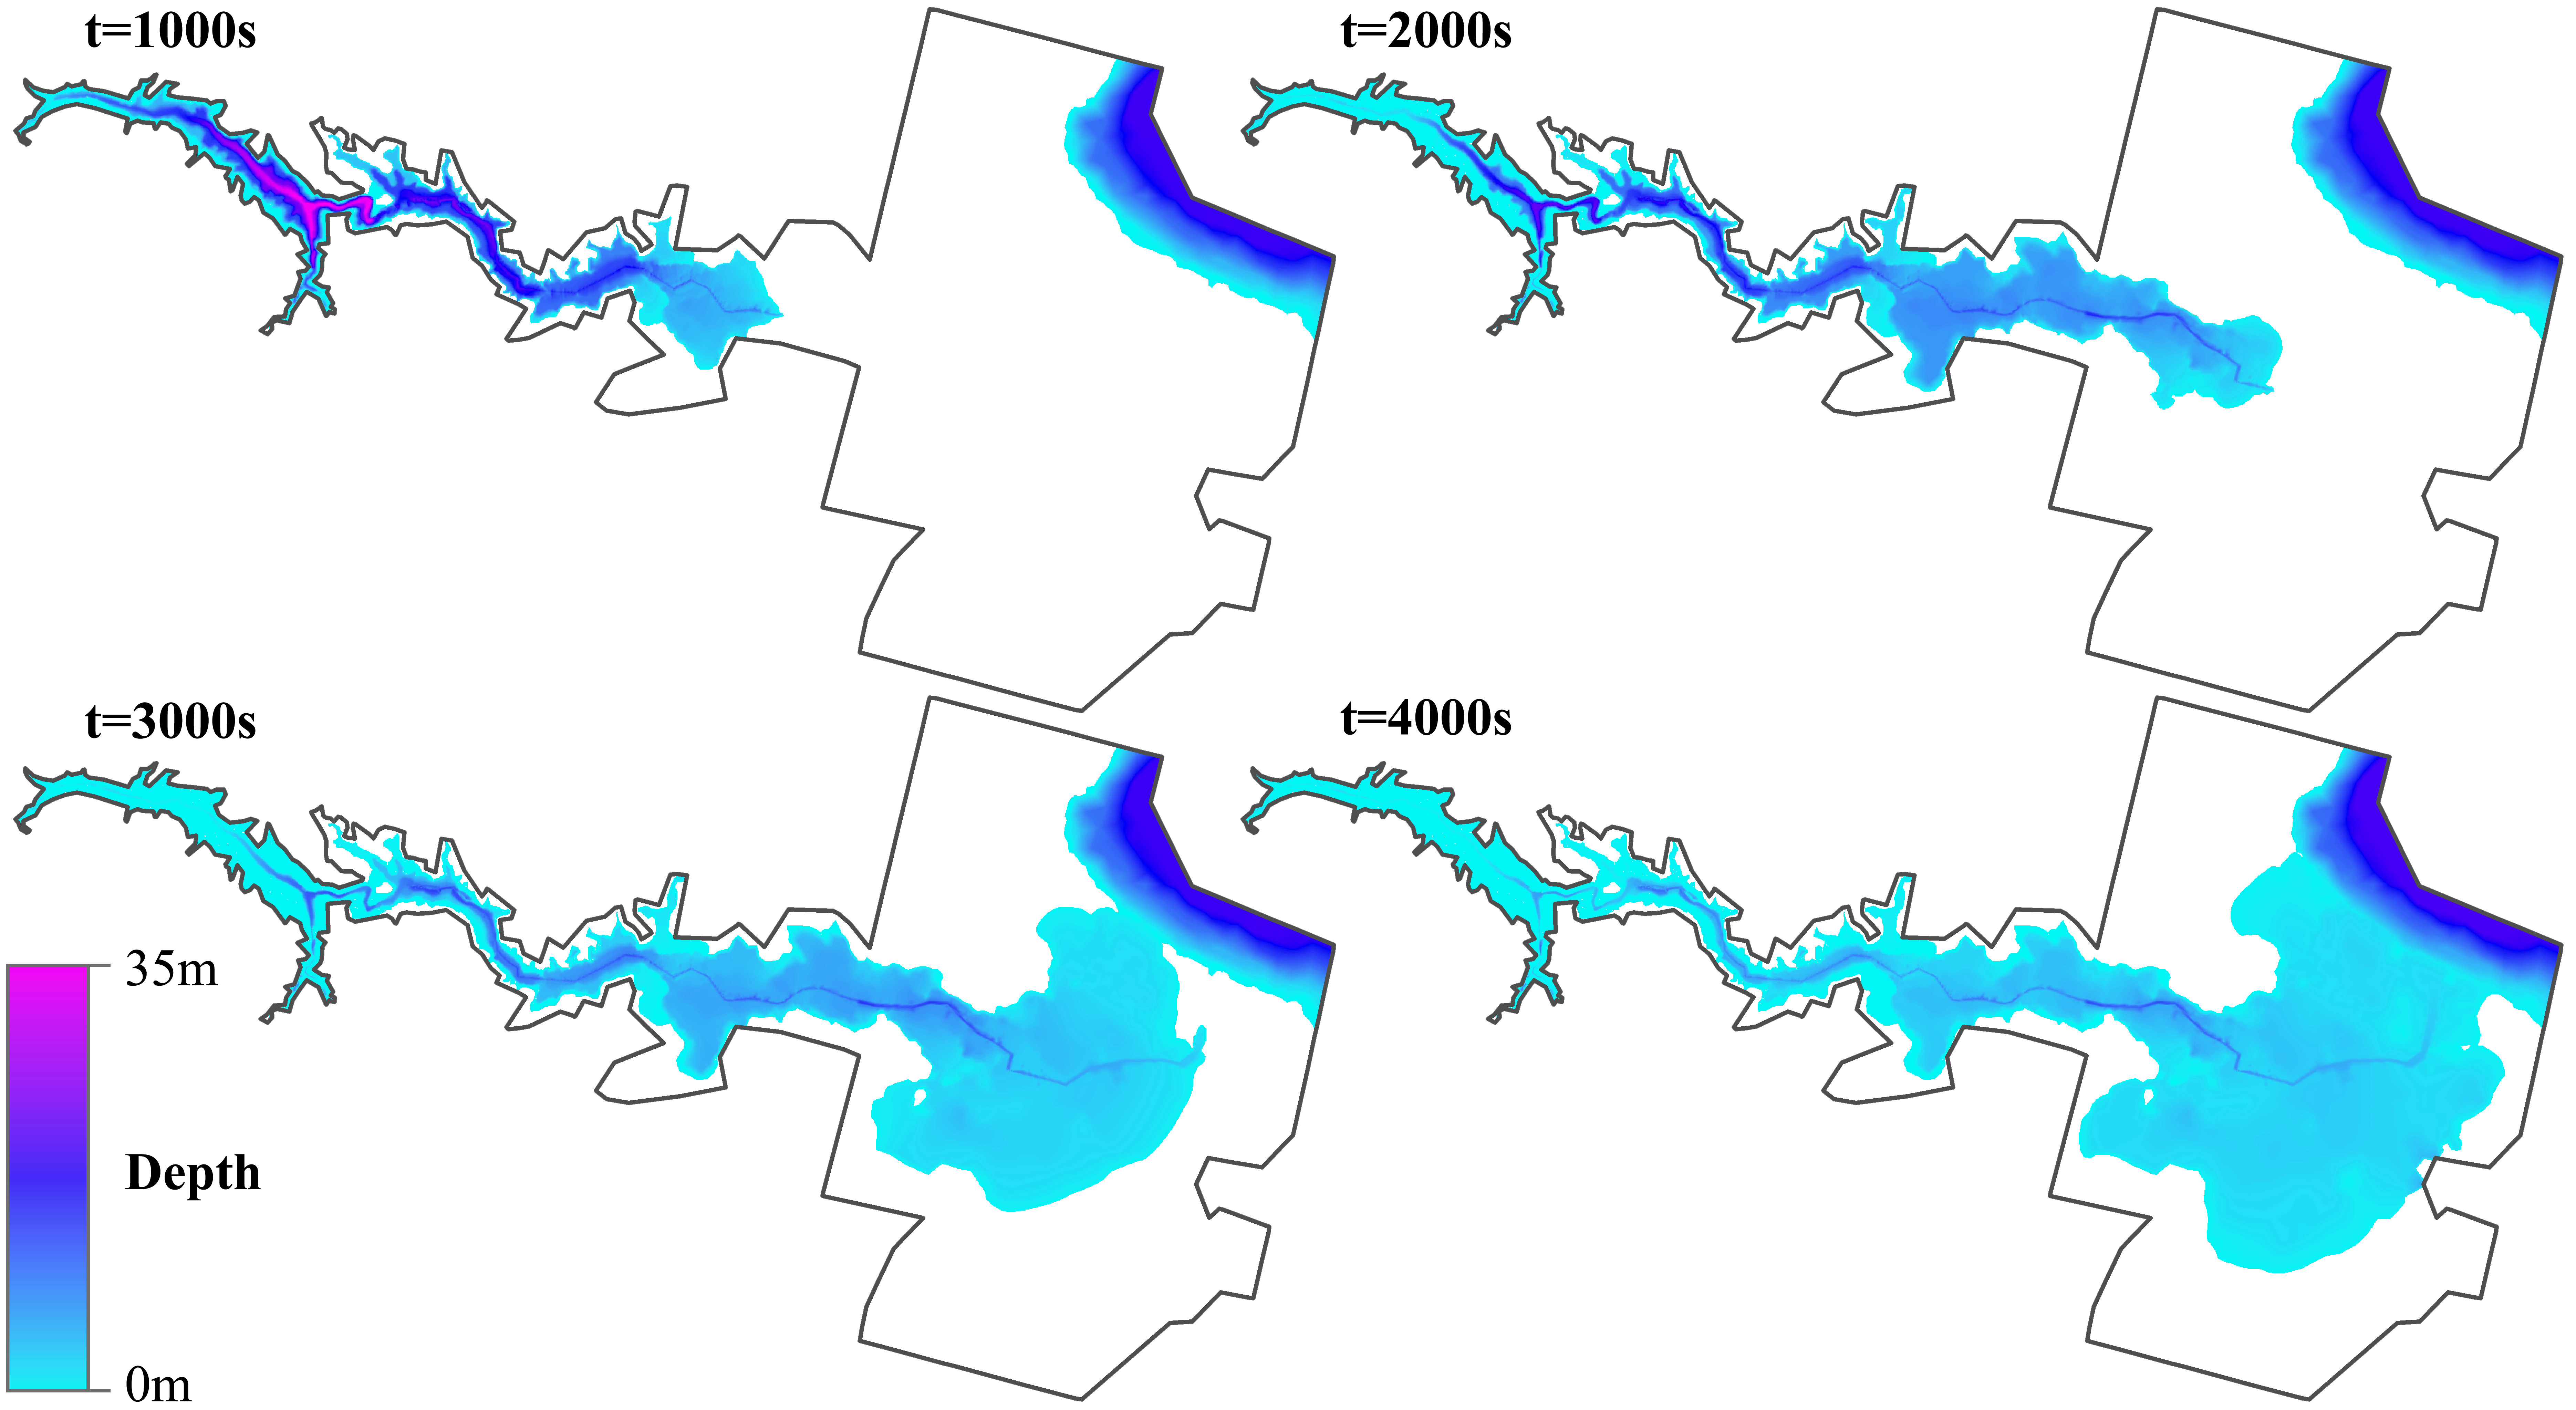
\includegraphics[width=0.8\textwidth]{Figure_9_Colour.jpg}
\caption{Evolving inundation map for the valley every 1000 seconds.}
\label{MalpassetProgression}
\end{figure*}
\begin{figure*}[tbh]
\centering
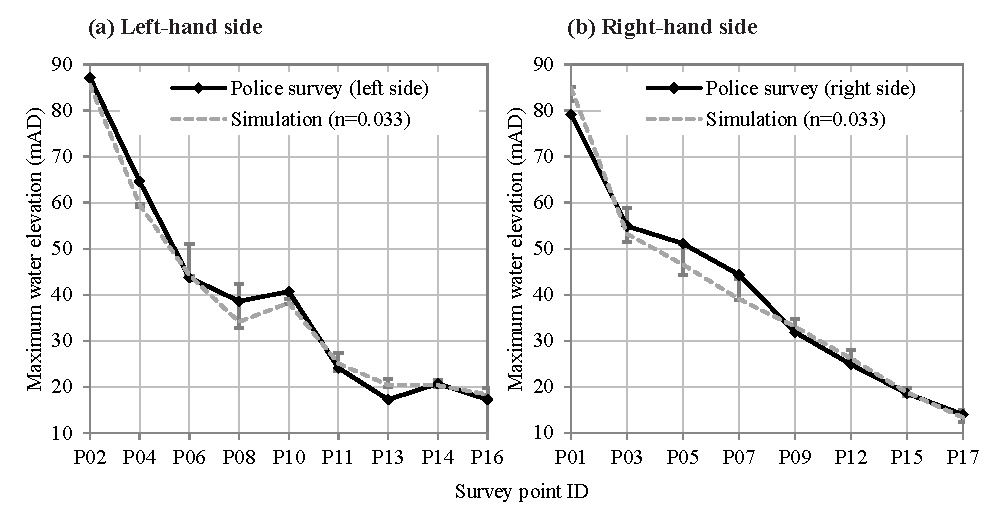
\includegraphics[width=0.9\textwidth]{Figure_10_Greyscale.pdf}
\caption{Comparison of maximum simulated free-surface levels on the left- and right-hand sides of the valley (looking downstream) against post-event police survey. Error bars indicate results for \(0.022 \le n \le 0.100\) }
\label{MalpassetValidation}
\end{figure*}
\begin{figure*}[tbh]
\centering
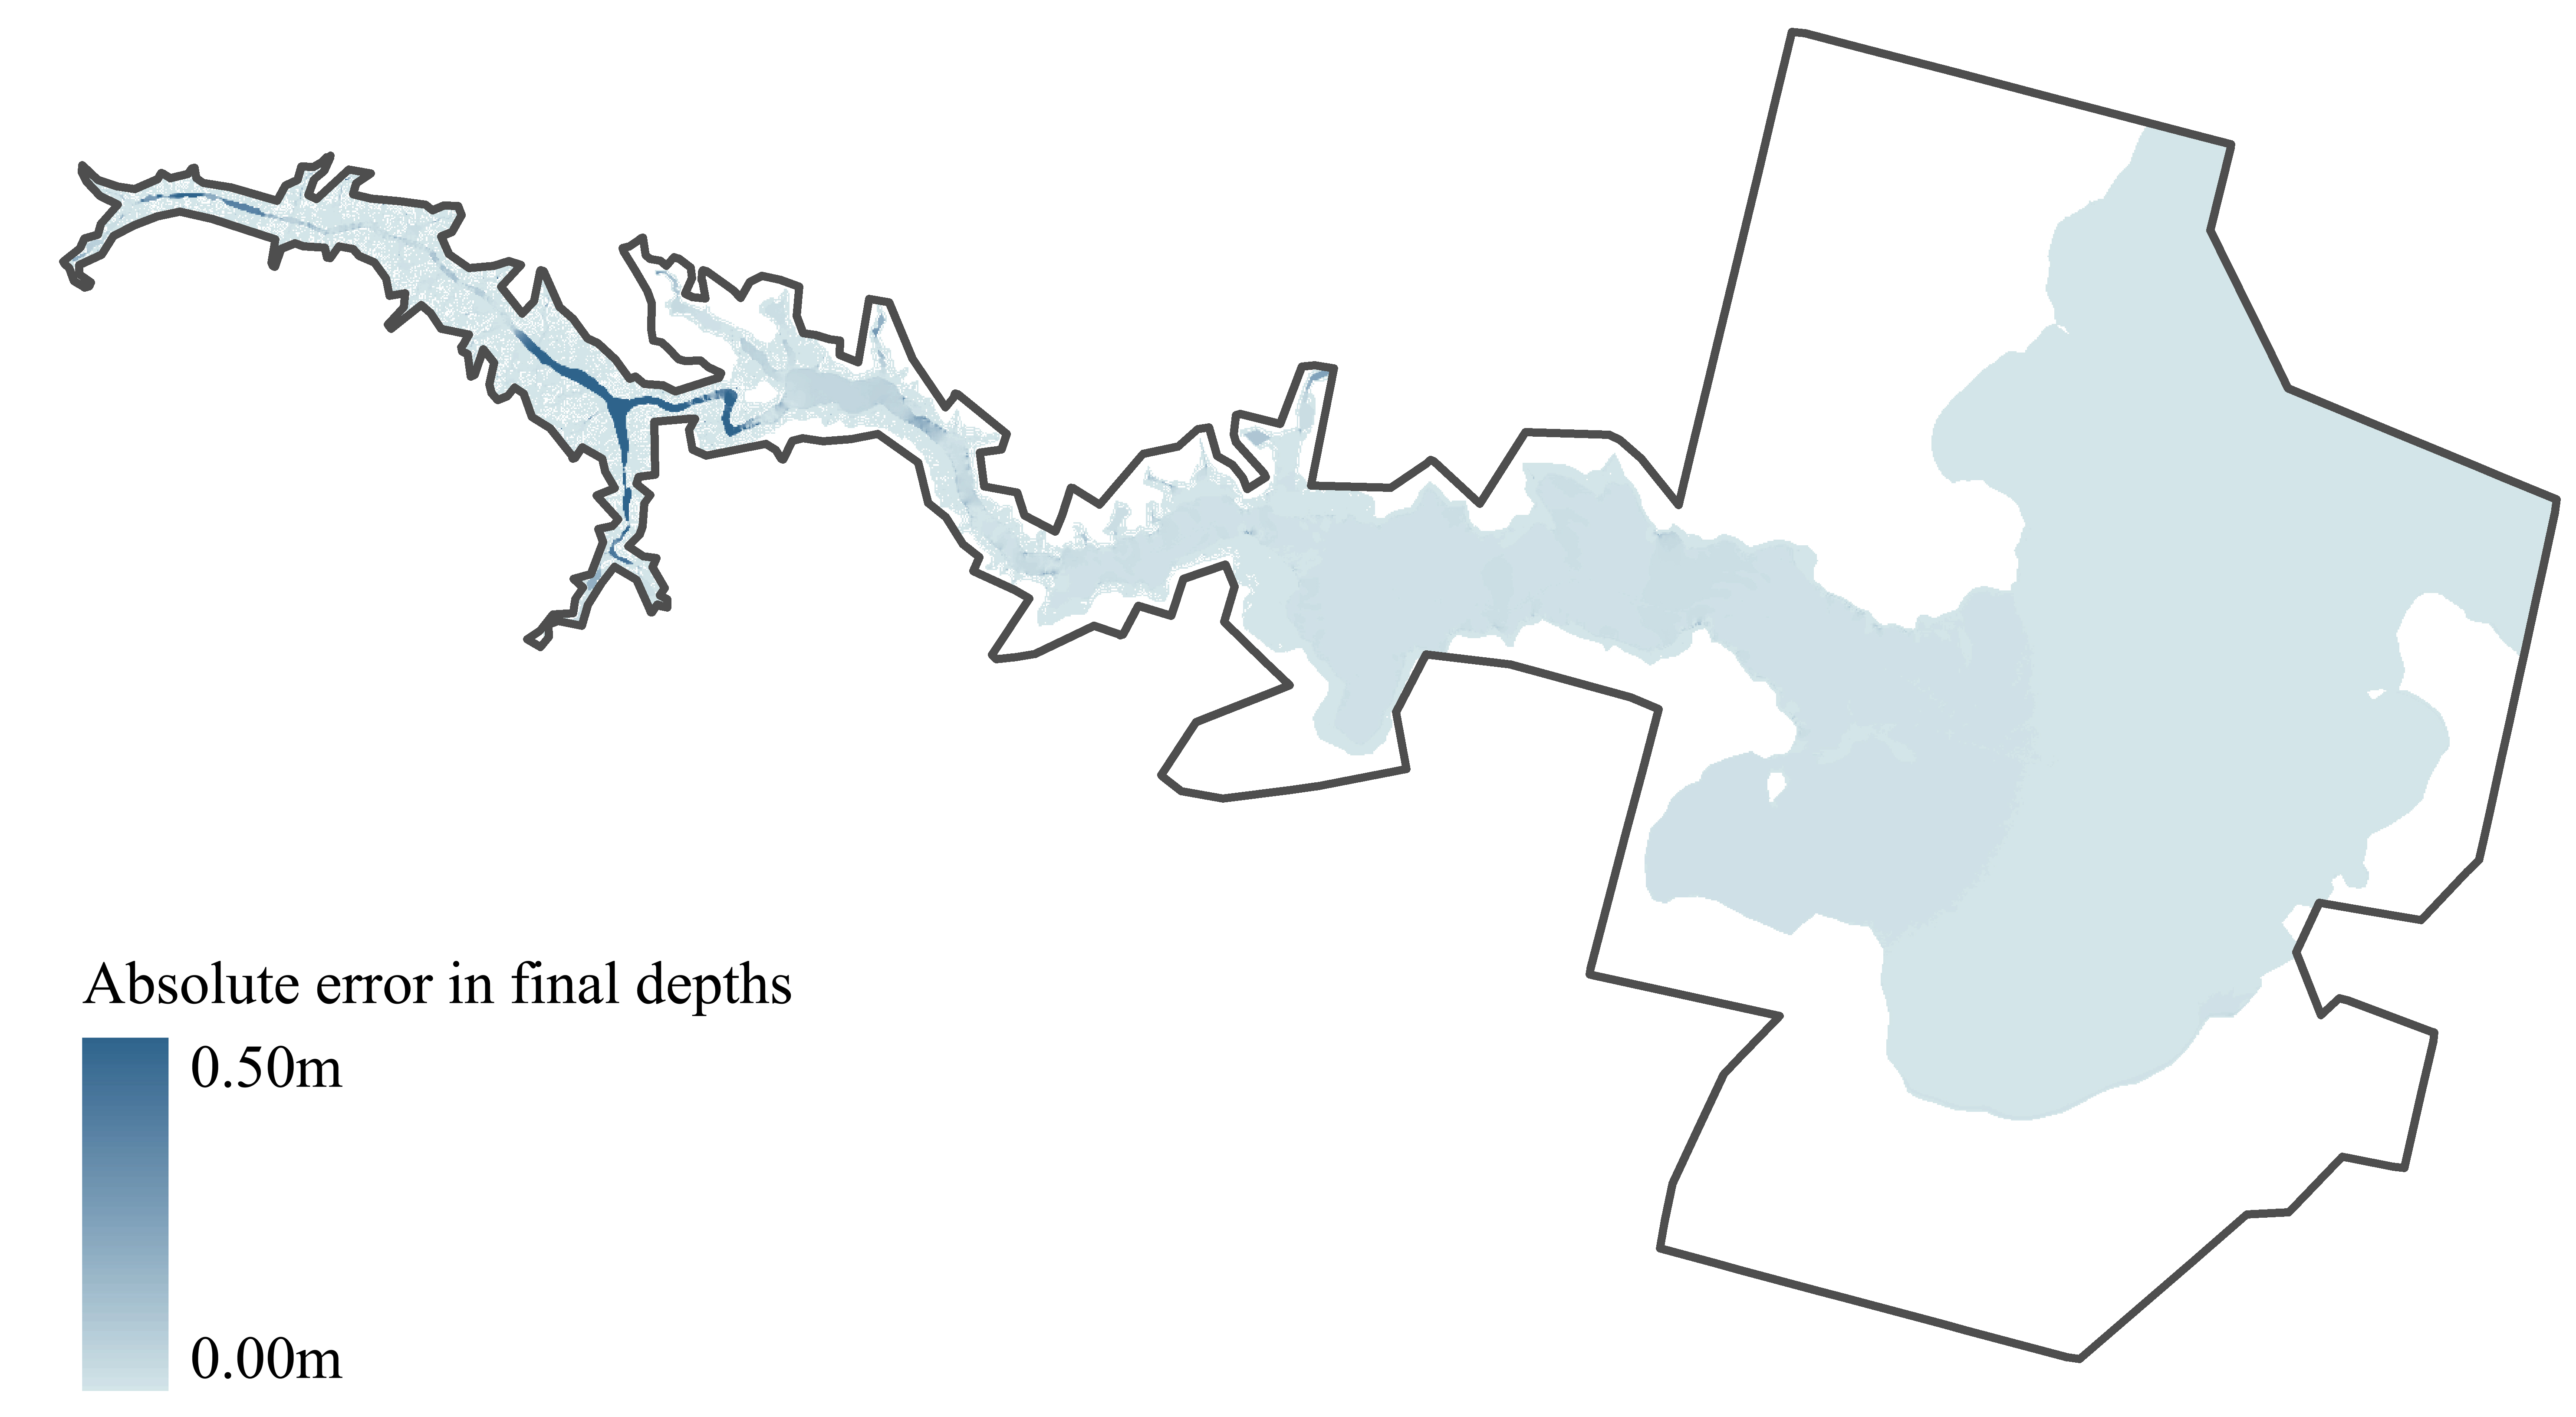
\includegraphics[width=0.7\textwidth]{Figure_11_Colour.jpg}
\caption{Spatial distribution of absolute errors introduced in the final depths (4000s) by using 32-bit floating-point after the Malpasset collapse, when compared to 64-bit results.}
\label{FPErrorFinal}
\end{figure*}
\begin{figure*}[tbh]
\centering
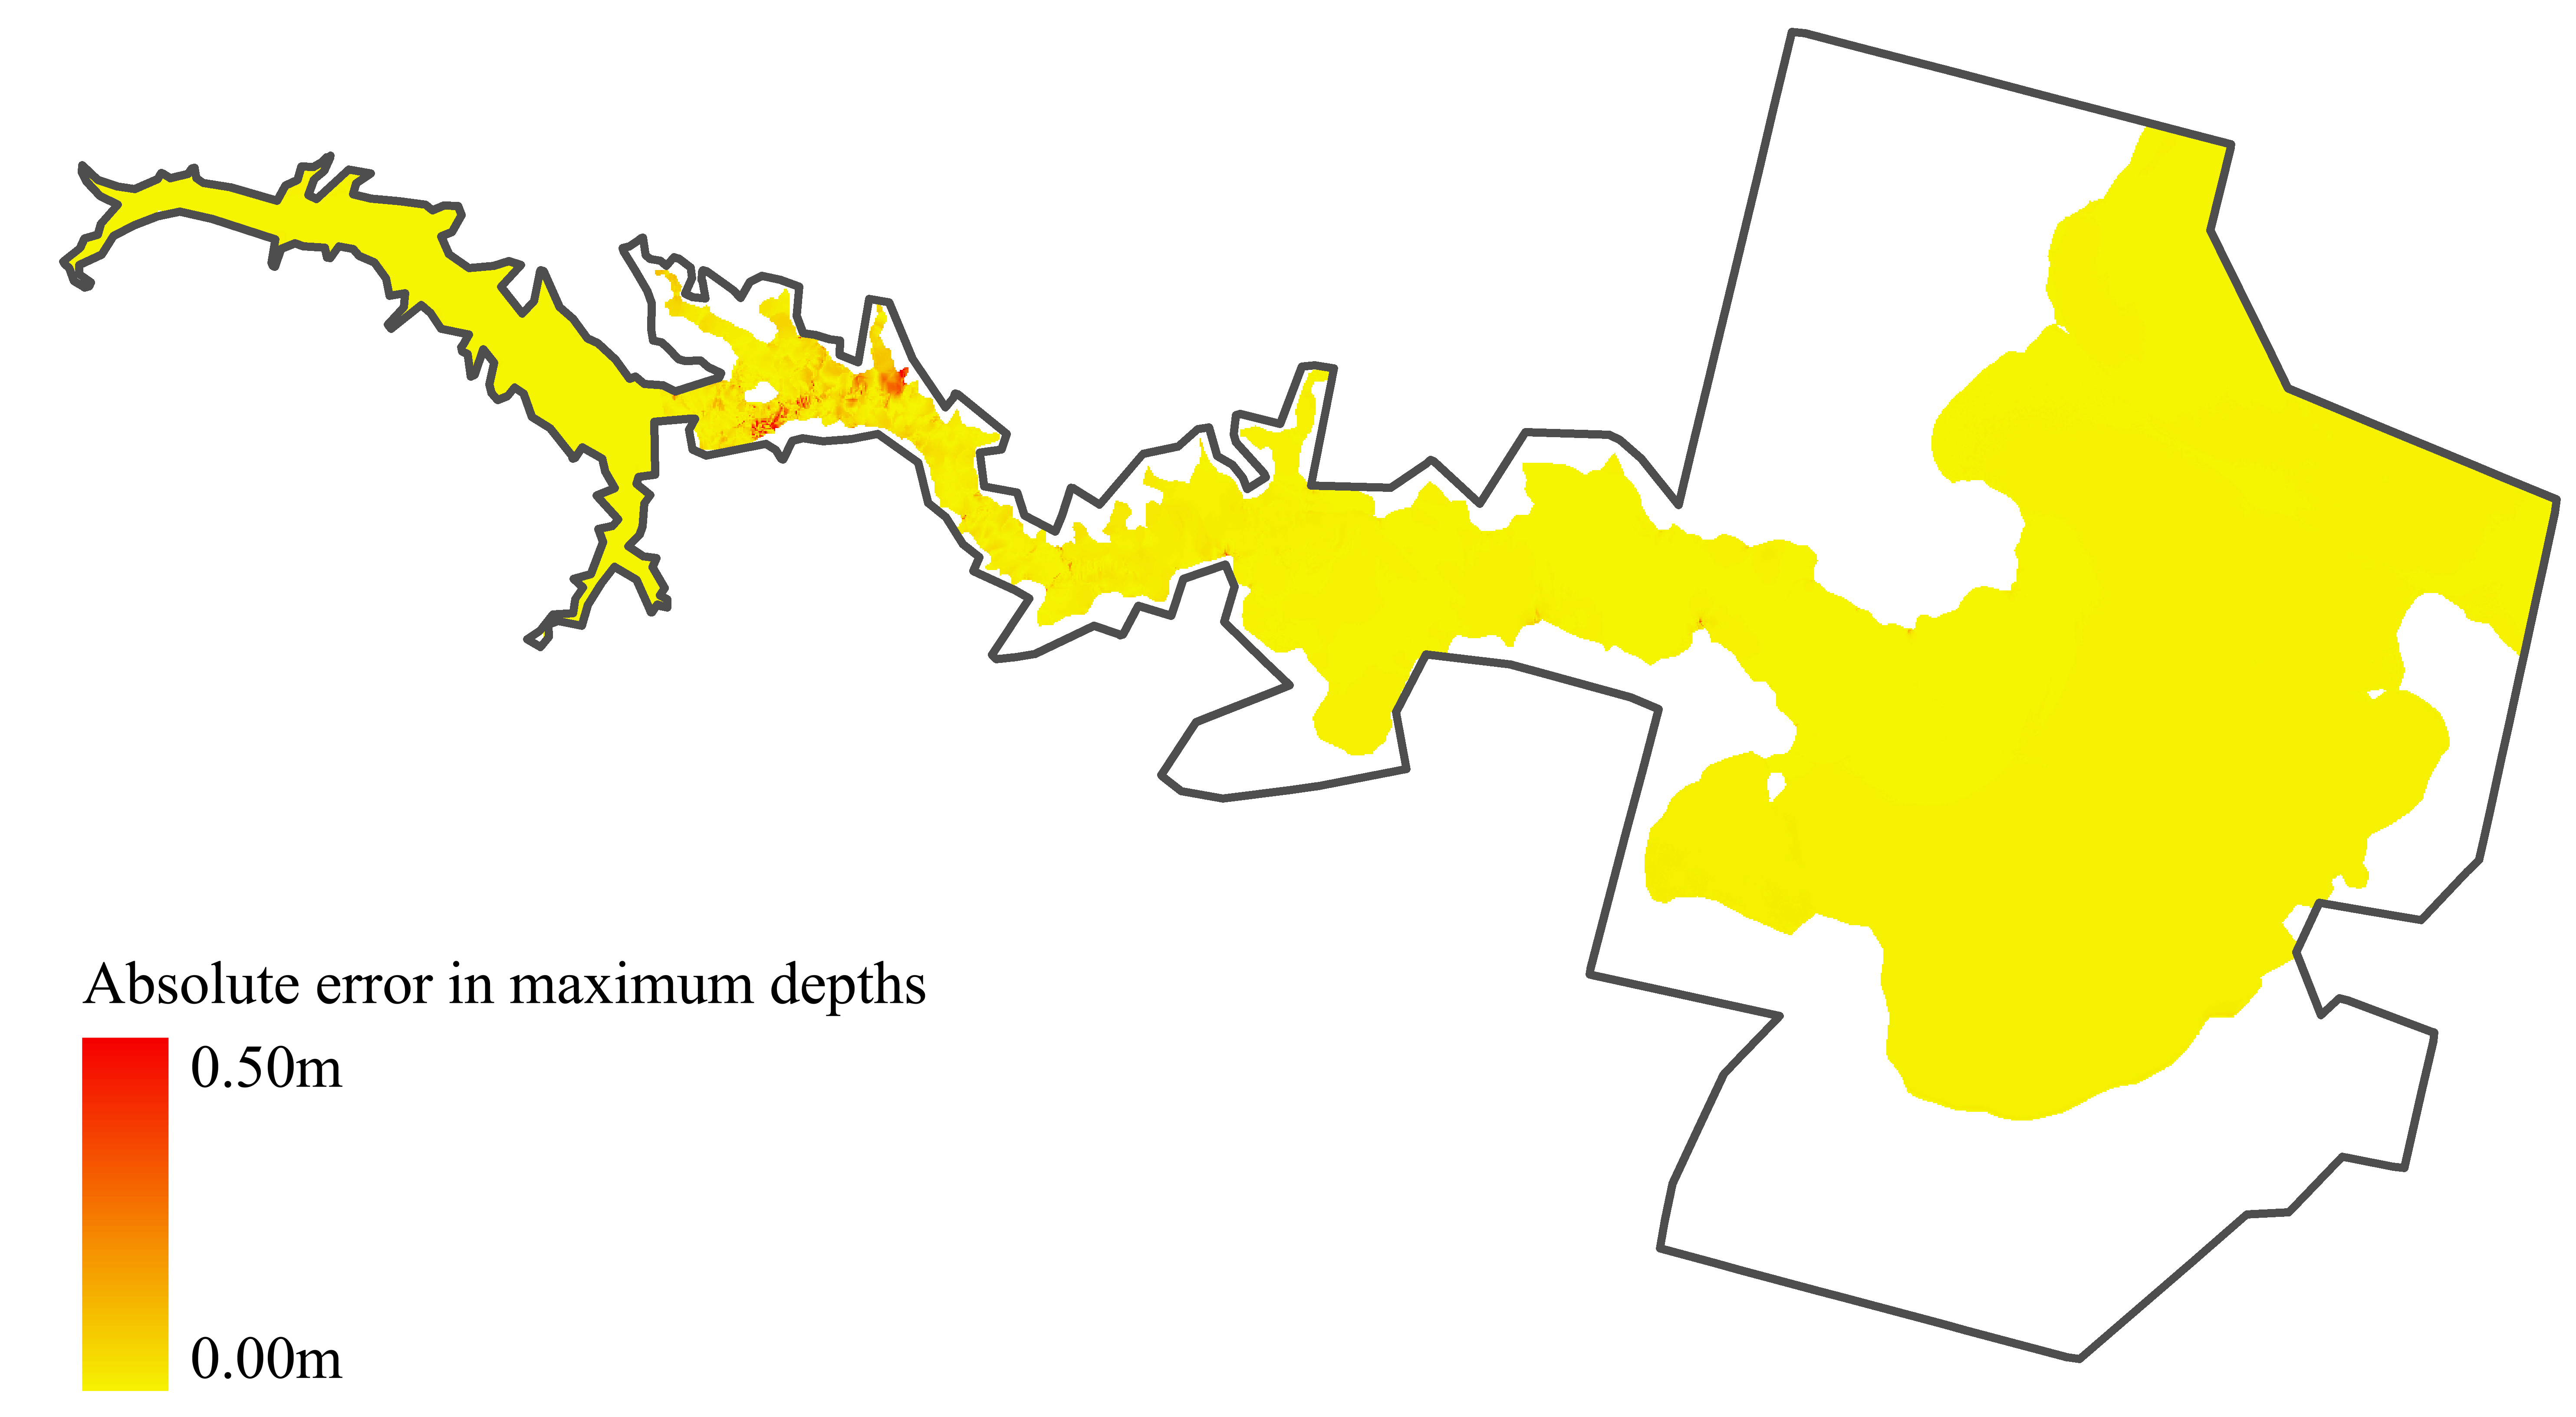
\includegraphics[width=0.7\textwidth]{Figure_12_Colour.jpg}
\caption{Spatial distribution of absolute errors introduced in the maximum depths by using 32-bit floating-point after the Malpasset collapse, when compared to 64-bit results.}
\label{FPErrorMax}
\end{figure*}

The memory model adopted in OpenCL is composed of private (i.e. registers), local (or LDS), and global (including constant) memory; Fig. \ref{OpenCLStructure} is a simplified representation of these memories. Global memory is the largest resource in which all data that persists throughout the simulation must reside. Scientific GPUs presently offer up to 6GB of global memory.

The scheme used herein is directionally unsplit, thus both axes are considered simultaneously by kernels. A first-order solution is therefore dependent on data from four neighbouring cells, but a second-order solution is dependent on data from twelve cells, which as demonstrated in Fig. \ref{RequisiteCellData} requires accessing global arrays using irregular strides. An alternative solution that reduces global accesses per cell is to commit cell data to local memory, synchronise the work-group, and subsequently access only that resource for neighbour data. 

The minimum amount of local memory available for devices conformant to the OpenCL specification is 32kB (some devices have 48kB available), but maintaining activity on at least four work-groups requires each kernel to consume 8kB or less of local memory. Committing cell data for the whole work-group to local memory using a typical GPU work-group size of 256 hence allows for only 32 bytes of data per cell (i.e. four double-precision values).  This is insufficient to store four sets of cell face-extrapolated half-timestep advanced values. Moreover, cells towards the extremity of a work-group cannot be solved using the data in the local cache because neighbours are absent, so work-groups are required to overlap and the global work size is increased accordingly. Without caching, the whole work-group can be considered productive and no overlap is required. Caching for a prediction kernel requires a single layer overlap and increases the global work size by 30\% for a work-group size of 256, whereas caching for the whole computation in a single kernel is both arithmetically intensive and requires a double layer overlap, drastically increasing the global work size by 78\%. To address these constraints in this work, face-extrapolated data are held only in global or private memory depending on the configuration. Similarly, conserved variables may be configured as cached to local memory or read directly from global memory.

Finally, local memory on GPUs is divided into banks (typically 16 or 32); serialisation is required for accesses to addresses in the same bank (i.e. conflicts). These can be avoided by manipulating the dimensions of the cache array to introduce padding, but the increased memory consumption may reduce the number of schedulable units running simultaneously.

\subsection{Kernel structure}

A kernel in OpenCL is executed over the global work (i.e. whole domain), within which there are work-groups of work-items, as shown in Fig. \ref{OpenCLExecStructure}. A different work-item therefore handles each cell in the domain with reference to data held for neighbouring cells. For a GPU, work-groups are decomposed to schedulable units of wavefronts (AMD) or warps (NVIDIA) for execution; specifics and vendor differences can be found in \cite{AMD_11,NVIDIA_10,NVIDIA_10a,KhronosOpenCL_12}. Each processing unit should be constantly engaged in productive computation to achieve the best performance with GPU architectures, known as the level of occupancy. It requires that each processing unit is assigned multiple schedulable units, allowing high-latency operations (e.g. global memory accesses, which are equivalent to hundreds of clock cycles \cite{NVIDIA_10}) to be masked by the device's scheduling. Occupancy generally benefits from a high ratio of arithmetic operations to global data accesses but scheduling further units delivers no further benefit once a high occupancy is already achieved \cite{AMD_11}. Consequently there is no panacea for optimisation on every device when transposing the numerical scheme to kernels.

To achieve high efficiency regardless of vendor differences, user-selectable kernel configurations are implemented to explore the effects of memory access patterns, illustrated in Fig. \ref{Kernels} alongside the data stencils for each kernel. Configuration A is expected to perform well for devices with a high occupancy and sufficient resources to maintain enough warps/wavefronts to mask global memory latency, thus makes no use of local caching; configuration B introduces some caching to configuration A where possible in the half-timestep kernel, reducing the number of global accesses with irregular strides; and configuration C uses the maximum amount of caching and the least amount of global accesses, but the consequence is a greater computational burden because the half-timestep calculation must be repeated many times given that local memory is insufficiently sized to cache face extrapolated data. All high-end devices are expected to have enough resources (mainly registers) to perform best with configuration A. 

\subsection{Timestep reduction}

A single timestep is used for all cells, identified from the smallest permissible timestep in the domain. A kernel that iterates through every cell serially is highly inefficient (Amdahl's Law), hence a two-stage reduction is used here to capitalise on the parallel nature and power of the processing units. A fixed global work size is selected and used as the stride through the global array of cell data, with each work-item identifying the smallest timestep from those cells it examines. Each work-item commits this data to an array in local memory and binary comparison is carried out within each work-group, starting at the middle, progressing towards the first element, with work-items successively retired. The first work-item in a work-group commits the lowest timestep identified in the group to a much smaller global array, which is examined by the single instance of the kernel for advancing the overall simulation time. This process is represented in Fig. \ref{ReductionProcess}. The global work size provides a method of controlling the workload assigned to each work-item.

\subsection{Kernel scheduling and reduction control}

A small overhead is associated with executing kernels and receiving notification of completion with blocking commands or callbacks. This is alleviated by adding multiple iterations of the numerical scheme to the execution queue and only displaying progress feedback periodically. Consequently, kernels are occasionally queued unnecessarily, as the simulation cannot progress further until output files are written; in such cases the timestep reduces to zero and kernels will exit early. The main loops operating on the compute device and host computer to coordinate this are shown in Fig. \ref{ComputerDeviceInteraction}, where there will be numerous iterations of the OpenCL loop before returning to the host computer loop.

\section{Results and discussion}

Validation of individual elements of the numerical scheme against analytical results for standard test cases can be found elsewhere in literature \cite{Liang_10,Liang_09}, hence this section will focus on evaluating the performance benefits achieved through GPU processing. The results were obtained using an AMD FirePro V7800 GPU with 2GB of memory, an Intel Xeon E5-2609 2.40GHz quad-core CPU with access to 24GB of memory, and an NVIDIA Tesla M2075 GPU with 6GB of memory. The value of \(g\) is taken to be 9.81ms\(^{-2}\). Comparisons are drawn between three different hardware devices from each of the mainstream manufacturers for the same numerical scheme and codebase. Timestep reduction is carried out using 200 work-groups of the maximum size each device will support.

As a uniquely natured event, the Malpasset dam-break is frequently used as a validation test-case for shock-capturing hydraulic models \cite{Goutal_99}. The double-curvature arch-dam at Malpasset in the south of France failed catastrophically on the 2nd December 1959 at 9:14PM as it approached full capacity during a period of prolonged and intense rainfall. Almost 55,106m\(^{3}\) of water was released downstream towards Fr{\'e}jus, resulting in over 400 deaths. Data is available from a post-event police survey of the extent and a scale model constructed by EDF. The positions of transformers and high-water marks in the valley, plus gauges in the scale model, are indicated in Fig. \ref{MalpassetIntro}. A regular Cartesian grid of 10m resolution is used to represent the 18km \(\times\) 10km domain (1.8M cells). The initial free-surface level behind the dam is 100mAD (estimated ±0.5m error), and sea level 0mAD. Comparison of results on the left- and right-hand sides of the valley are presented in Fig. \ref{MalpassetValidation} for \(n=0.033\) (\(M=30\)), the value suggested by CADAM project participants.  The first 4000 seconds following the collapse are simulated. Fig. \ref{MalpassetProgression} shows the inundation extent in the valley at \(t=1000\), \(t=2000\), \(t=3000\), and \(t=4000\) seconds.

\subsection{CPU-GPU comparison}

The run-times with multiple configurations of the software developed herein are presented in Table \ref{PerformanceResults} for the different hardware. The results indicate that for 64-bit computation the NVIDIA GPU model can simulate the Malpasset collapse 6.3x faster than the Intel CPU, while the manufacturer-quoted peak performances suggest a 6.7x difference \cite{NVIDIA_11,Intel_12}; the actual and and quoted performance differences for the AMD device are 4.2 and 5.2 respectively \cite{AMD_12}. This is not altogether surprising; further analysis suggests the AMD device with 64-bit floating-point does not achieve full occupancy because the number of registers constrains the number of wavefronts. Nonetheless the AMD simulation time represents a significant improvement over the CPU, for a fraction of the cost of an NVIDIA Tesla GPU. Vendor-quoted peak performance levels are rarely achievable in practical applications and are compared only to give an indication of device processing power. For users without a suitable GPU the software will nevertheless provide a significant performance boost, given that the new software fully harnesses all four cores of the CPU at all stages of the numerical scheme, unlike most existing commercial software.

Caching data to local memory provides no performance benefit with 32- or 64-bit floating-point computation for any of the devices tested herein. Where local memory is used however, oversizing the array is often shown to improve performance by alleviating bank conflicts. 

\subsection{Effects of floating-point precision}

In all simulations carried out 32-bit computation was faster than 64-bit. There are substantial and significant differences in the results obtained however, which demonstrate that 32-bit introduces unacceptably large errors. The spatial distribution of errors in the final and maximum simulated depths are shown in Fig. \ref{FPErrorFinal} and Fig. \ref{FPErrorMax} respectively.  Errors in maximum depth are concentrated in areas with the greatest flow velocities and where shocks are observed immediately downstream of the dam, whereas the final depth errors mainly lie in the shoal zones of the catchment where water should drain. While the mean error in final depths with SP is \(<0.05\)m, the greatest error was \(+1.89\)m, and for the maximum depths the greatest error was \(+0.85\)m. The technique adopted herein uses free-surface level as a conserved variable instead of depth, which reduces the numerical resolution of shallow depths in particular. Whilst the localised errors may be a by-product of the specific numerical scheme employed herein, we urge caution and encourage further research before 64-bit precision is dispensed with for performance over accuracy.

Other authors have previously reported the differences between 32- and 64-bit floating-point in terms of a mass balance error introduced by successive rounding (e.g. \cite{Brodtkorb_10}), which potentially overlooks the significant magnitude of localised errors. Unlike this study they conclude that 32-bit floating-point provides an acceptable degree of accuracy. This difference stems from the different numerical scheme employed herein. Mixing different levels of precision remains a possibility. 

\section{Conclusions}

In this paper, we have presented how the shallow water equations can be efficiently solved with second-order accuracy using a finite-volume Godunov-type scheme and GPUs. Factors affecting GPU performance are considered and a range of corresponding configuration parameters devised to allow the software to be used and optimised with a wide range of modern processors. Simulations of a real-world dam collapse event with the new framework were shown to exhibit good agreement with a post-event survey, without compromising accuracy but still providing significant performance improvements against a CPU. The results demonstrate that the software developed herein is appropriate for simulating some of the most challenging flood events, where shock-like flow discontinuities are present. The new approach will facilitate simulations at resolutions previously unfeasible across whole cities and large catchments. As further work, we propose to extend the software to take advantage of multiple GPUs in a single host computer to facilitate further performance improvements and greater numbers of cells.

32-bit floating-point simulations are shown to introduce significant but localised errors to results; 64-bit is therefore recommended for flood modelling. Caching cell data to local memory provided no direct performance benefit for any of the devices used. Where local memory is used, reducing bank conflicts with array padding is shown to reduce simulation times slightly.

\section*{Acknowledgements}
This work was generously supported by Advanced Micro Devices, Inc. who provided the ATI FirePro V7800 GPU devices used for the study. The authors also acknowledge the support of EPSRC through small equipment grants (EP/K031678/1) and doctoral training account.

\bibliographystyle{apalike}
\bibliography{GPUPaper01}

\end{document}